%!xelatex = 'xelatex --halt-on-error %O %S'

\documentclass{thuemp}
\begin{document}

% 标题,作者
\emptitle{Week 9}
\empauthor{Jacob}{2019011325}

% 奇数页页眉 % 请在这里写出第一作者以及论文题目
\fancyhead[CO]{{\footnotesize 江灿: 光栅衍射实验报告}}


%%%%%%%%%%%%%%%%%%%%%%%%%%%%%%%%%%%%%%%%%%%%%%%%%%%%%%%%%%%%%%%%
% 关键词 摘要 首页脚注
%%%%%%%%关键词



\maketitle

%%%%%%%%摘要

% \empfirstfoot{2022-04-03}{软件02}{双日下M}{7号}
%%%%%%%%首页角注,依次为实验时间、报告时间、学号、email


%%%%%%%%!首页角注可能与正文重叠,请通过调整正文中第一页的\enlargethispage{-3.3cm}位置手动校准正文底部位置:
%%%%%%%%%%%%%%%%%%%%%%%%%%%%%%%%%%%%%%%%%%%%%%%%%%%%%%%%%%%%%%%%
%  正文由此开始
\wuhao 
%  分栏开始

\section*{Step 1}
let educated people go where they want to go; it is suitable for both people and the country they belong to.

\section*{Step 2 : benefits}
\begin{itemize}
  \item migrants repay by remitted; some are huge.
  \item help well-educated emigrants find jobs

  \item can give developing countries an incentive to invest in education.

  \item can affect the home country directly by shaping the regulatory structure of the home country's venture-capital
  

\end{itemize}

\section*{Step 3 }
I think this argument is vital in using data rather than subjective assumptions, such as the remitted, which use the exact number of the remitted of \$325 in 2010, and the more than 20\%GDP. Their number shows 
the thing in the true in the world. But I also think there is a weak place as to how the migration decamping to Silicon Valley, Which causes the 
loss of the home country, will do the wrong thing to the home country. If there is evidence that can compare the loss of migration and the repayment, the statistics will be better.
%%%%%%%%%%%%%%%%%%%%%%%%%%%%%%%%%%%%%%%%%%%%%%%%%%%%%%%%%%%%%%%%

%%%%%%%%%%%%%%%%%%%%%%%%%%%%%%%%%%%%%%%%%%%%%%%%%%%%%%%%%%%%%%%%

\newpage
% \begin{figure}[H]
% 	\centering
% 	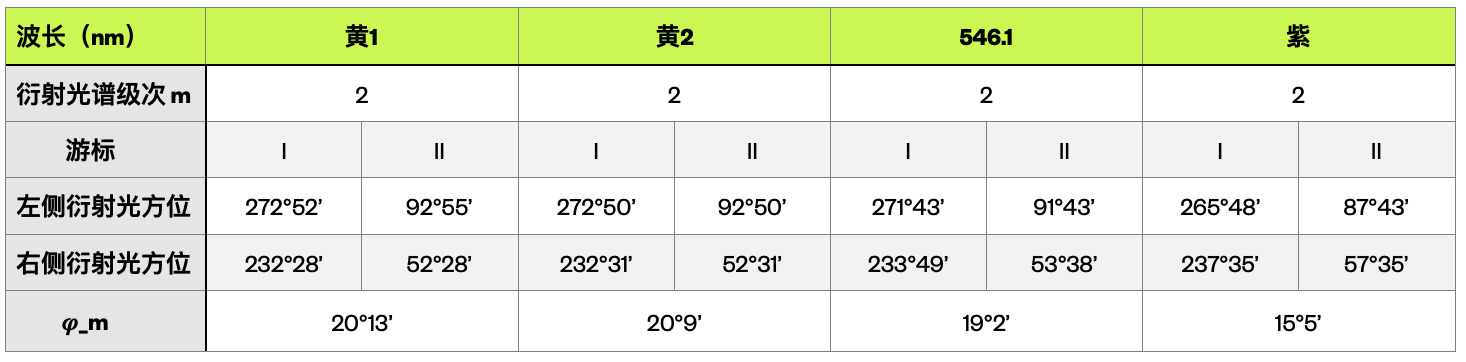
\includegraphics[width=0.8\linewidth]{./image/1.png}
% 	\caption{测定光栅常数和光波波长数据} 
% 	\label{png:1}
% \end{figure}








%%%%%%%%%%%%%%%%%%%%%%%%%%%%%%%%%%%%%%%%%%%%%%%%%%
%  参考文献
%%%%%%%%%%%%%%%%%%%%%%%%%%%%%%%%%%%%%%%%%%%%%%%%%%%%%%%%%%%%%%%%
%  参考文献按GB/T 7714-2015《文后参考文献著录规则》的要求著录. 
%  参考文献在正文中的引用方法:\cite{bib文件条目的第一行}

\renewcommand\refname{\heiti\wuhao\centerline{参考文献}\global\def\refname{参考文献}}
\vskip 12pt

\let\OLDthebibliography\thebibliography
\renewcommand\thebibliography[1]{
  \OLDthebibliography{#1}
  \setlength{\parskip}{0pt}
  \setlength{\itemsep}{0pt plus 0.3ex}
}

{
\renewcommand{\baselinestretch}{0.9}
\liuhao
\bibliographystyle{gbt7714-numerical}
\bibliography{./TempExample}
}


\end{document}
